\documentclass[en,t]{sdqbeamer}

\usepackage{amssymb} %% For \backprime
\usepackage{multicol}

%\usepackage{mathpartir}
\usepackage{graphicx}

\usepackage{tikz}
\usetikzlibrary{arrows.meta,positioning,calc}

\usepackage[style=authoryear,backend=bibtex]{biblatex}
\bibliography{lean}

\usepackage[T1]{fontenc}
\usepackage{babel}
\usepackage{booktabs}
\usepackage[normalem]{ulem}
\usepackage{fontspec}
\setmonofont[Scale=MatchLowercase]{Iosevka}
%\newfontfamily\lc[Scale=MatchLowercase]{Iosevka SS09}
%
%%%%%%%%%%%%%%%%%%%%%%%%%%%%%%%%%%%%%%%%%%%%%%%%%%%%%%%%%%%%%%%%%%%%%%%%%%%%%%%
% Add minted and support costum lexers
%%%%%%%%%%%%%%%%%%%%%%%%%%%%%%%%%%%%%%%%%%%%%%%%%%%%%%%%%%%%%%%%%%%%%%%%%%%%%%%
\usepackage{minted}
\makeatletter
\ifwindows
  \renewcommand{\minted@optlistcl@quote}[2]{%
    \ifstrempty{#2}{\detokenize{#1}}{\detokenize{#1="#2"}}}
\else
  \renewcommand{\minted@optlistcl@quote}[2]{%
    \ifstrempty{#2}{\detokenize{#1}}{\detokenize{#1='#2'}}}
\fi

% similar to \minted@def@optcl@switch
\newcommand{\minted@def@optcl@novalue}[2]{%
  \define@booleankey{minted@opt@g}{#1}%
    {\minted@addto@optlistcl{\minted@optlistcl@g}{#2}{}%
     \@namedef{minted@opt@g:#1}{true}}
    {\@namedef{minted@opt@g:#1}{false}}
  \define@booleankey{minted@opt@g@i}{#1}%
    {\minted@addto@optlistcl{\minted@optlistcl@g@i}{#2}{}%
     \@namedef{minted@opt@g@i:#1}{true}}
    {\@namedef{minted@opt@g@i:#1}{false}}
  \define@booleankey{minted@opt@lang}{#1}%
    {\minted@addto@optlistcl@lang{minted@optlistcl@lang\minted@lang}{#2}{}%
     \@namedef{minted@opt@lang\minted@lang:#1}{true}}
    {\@namedef{minted@opt@lang\minted@lang:#1}{false}}
  \define@booleankey{minted@opt@lang@i}{#1}%
    {\minted@addto@optlistcl@lang{minted@optlistcl@lang\minted@lang @i}{#2}{}%
     \@namedef{minted@opt@lang\minted@lang @i:#1}{true}}
    {\@namedef{minted@opt@lang\minted@lang @i:#1}{false}}
  \define@booleankey{minted@opt@cmd}{#1}%
      {\minted@addto@optlistcl{\minted@optlistcl@cmd}{#2}{}%
        \@namedef{minted@opt@cmd:#1}{true}}
      {\@namedef{minted@opt@cmd:#1}{false}}
}

\minted@def@optcl@novalue{customlexer}{-x}
\makeatother
\definecolor{codebg}{rgb}{0.95,0.95,0.95}
\setminted{bgcolor=codebg,breaklines}
\usemintedstyle{tango}
\newmintinline[lean]{lean4.py:Lean4Lexer}{customlexer=true, bgcolor=white}
\newminted[leancode]{lean4.py:Lean4Lexer}{customlexer=true, fontsize=\footnotesize}

\usepackage{newunicodechar}
\newfontfamily{\freeserif}{DejaVu Sans}
\newunicodechar{ℕ}{\freeserif{ℕ}}
\newunicodechar{ℝ}{\freeserif{ℝ}}
\newunicodechar{ₐ}{\freeserif{ₐ}}
%\newunicodechar{₁}{\freeserif{₁}}
%\newunicodechar{∈}{\freeserif{∈}}
\newunicodechar{𝓞}{\ensuremath{\mathcal{O}}}
\newunicodechar{∉}{\freeserif{∉}}
%\newunicodechar{Π}{\freeserif{Π}}
%\newunicodechar{→}{\freeserif{→}}
\newunicodechar{⦃}{\freeserif{⦃}}
\newunicodechar{⦄}{\freeserif{⦄}}
%\newunicodechar{∧}{\freeserif{∧}}
%\newunicodechar{∨}{\freeserif{∨}}
%\newunicodechar{⊢}{\freeserif{⊢}}
\newunicodechar{⊑}{\freeserif{⊑}}
\newunicodechar{ₚ}{\freeserif{ₚ}}
\newunicodechar{∘}{\freeserif{∘}}
\newunicodechar{ₗ}{\freeserif{ₗ}}
\newunicodechar{∪}{\freeserif{∪}}
\newunicodechar{⋃}{\freeserif{⋃}}
\newunicodechar{𝓸}{\ensuremath{o}}
\newunicodechar{⊆}{\freeserif{⊆}}
\newunicodechar{≼}{\freeserif{≼}}
\newunicodechar{≃}{\freeserif{≃}}

% https://github.com/gpoore/minted/issues/220
\AtBeginEnvironment{snugshade*}{\vspace{-0.4\FrameSep}}
%\AfterEndEnvironment{snugshade*}{\vspace{-0.8\FrameSep}}

% https://tex.stackexchange.com/questions/343494/minted-red-box-around-greek-characters
\makeatletter
\AtBeginEnvironment{minted}{\dontdofcolorbox}
\def\dontdofcolorbox{\renewcommand\fcolorbox[4][]{##4}}
\makeatother

\title{Syntax Extensibility in Lean 4}

\author[Ullrich]{Sebastian Ullrich}
\institute[IPD Snelting]{Programming paradigms group - IPD Snelting}
\date{2023/06/21}
\titleimage{logo}
\grouplogo{stlogo-600dpi}

\newcommand{\kit}[1]{\textcolor{kit-green}{#1}}

\begin{document}
\KITtitleframe

\begin{frame}{Towards a Fully Extensible Frontend}
  Goal: \emph{democratize} frontend by removing the barrier between built-in and user-defined notions
  \begin{itemize}
    \pause
  \item extensible syntax from simple mixfix notations to character-level parsing
    \pause
  \item extensible semantics from simple syntax sugars to type-aware elaboration
    \pause
  \item extensible tooling with access to frontend metadata
    \begin{itemize}
    \item concrete syntax tree
    \item elaboration annotations
    \end{itemize}
  \end{itemize}
  \pause
  \bigskip
  Non-goal: extensible type theory
\end{frame}

\begin{frame}[fragile]{Frontend: Overview}
    \begin{tikzpicture}[overlay,>=stealth, thick, nodes={rounded corners, minimum height=2em}, level distance=18mm]
      \node[draw] at (\textwidth/2,0) {language server}
      child[->] {
        node[draw] (parser) {parser}
        child {
          node[draw]  (elab) {elaborator}
          child[->] {
            node[draw] {kernel}
            edge from parent node[right] {core term}
          }
          edge from parent node[right] {concrete syntax tree}
        }
        edge from parent node[right] {string}
      };
      \draw[->,loop right] (elab) to node {concrete syntax tree} (elab);
    \end{tikzpicture}
\end{frame}

\begin{frame}[fragile]{Concrete Syntax Tree}
  provide
  \begin{itemize}
  \item precise source locations
  \item whitespace and comments
  \item erroneous input
  \end{itemize}
  for
  \begin{itemize}
  \item code editors
  \item documentation generators
  \item code formatters
  \item refactoring tools
  \item better LaTeX highlighting...
  \end{itemize}
\end{frame}

\begin{frame}[fragile,fragile]{Extensible Concrete Syntax Tree}
\begin{leancode}
inductive Syntax where
  | atom   (info : SourceInfo) (val : String)
  | ident  (info : SourceInfo) (rawVal : Substring) (val : Name) (preresolved : List Syntax.Preresolved)
  | node   (info : SourceInfo) (kind : SyntaxNodeKind) (args : Array Syntax)
  | missing

inductive SourceInfo where ...

abbrev SyntaxNodeKind := Name
\end{leancode}

\begin{leancode}
a -> b
\end{leancode}

\begin{leancode}
(Term.arrow `a "->" `b)
\end{leancode}
\end{frame}

\begin{frame}{Parser}
  \begin{itemize}
  \item Lean 3: basic lexer, LL(1) recursive descent parser
  \item Isabelle: basic lexer, Earley parser for arbitrary context-free grammars, delimited terms
    \pause
  \item Lean 4: arbitrary, character-based parser; combinators including Pratt
    parser and longest-prefix matching
    \pause
    \begin{itemize}
    \item problem: monadic parser combinators allocate like crazy, lexing and parsing should
      be cached
    \end{itemize}
  \end{itemize}
\end{frame}

\begin{frame}[fragile]{Parser State}
\begin{leancode}
def ParserFn := ParserContext → ParserState → ParserState

structure ParserContext where  -- simplified
  input    : String
  fileName : String
  fileMap  : FileMap
  env      : Environment
  prec     : Nat
  -- ...

structure ParserState where
  pos      : String.Pos
  stxStack : SyntaxStack
  cache    : ParserCache
  errorMsg : Option Error
  -- ...
\end{leancode}
\end{frame}

\begin{frame}[fragile,fragile,fragile]{Syntax Stack}
\begin{leancode}
def nodeFn (k : SyntaxNodeKind) (p : ParserFn) : ParserFn
\end{leancode}
  
\begin{leancode}
nodeFn `Term.arrow (identFn >> symbolFn "->" >> identFn)
\end{leancode}

\begin{leancode}
   [..., `a, "->", `b]
~> [..., (Term.arrow `a "->" `b)]
\end{leancode}
\end{frame}


\begin{frame}[fragile]{Token Caching}
  Cache last ``token'' read
\begin{leancode}
def tokenFn (expected : List String := []) : ParserFn := fun c s =>
  let input := c.input
  let i     := s.pos
  if input.atEnd i then s.mkEOIError expected
  else
    let tkc := s.cache.tokenCache
    if tkc.startPos == i then
      let s := s.pushSyntax tkc.token
      s.setPos tkc.stopPos
    else
      let s := tokenFnAux c s
      updateTokenCache i s
\end{leancode}
\end{frame}

\begin{frame}[fragile]{Token Caching}
  Token set not currently extensible except for constant-length symbols
\begin{leancode}
private def tokenFnAux : ParserFn := fun c s =>
  let input := c.input
  let i     := s.pos
  let curr  := input.get i
  if curr == '”' then
    strLitFnAux i c (s.next input i)
  else if curr == '\'' && getNext input i != '\'' then
    charLitFnAux i c (s.next input i)
  else if curr.isDigit then
    numberFnAux c s
  else if curr == '`' && isIdFirstOrBeginEscape (getNext input i) then
    nameLitAux i c s
  else
    let (_, tk) := c.tokens.matchPrefix input i
    identFnAux i tk .anonymous c s
\end{leancode}
  \pause
  Plan for unblocking incompatible lexical syntax: store \lean{tokenFnAux} in parser context, making it replaceable
\end{frame}

\begin{frame}[fragile]{Token Caching}
\begin{leancode}
def identFn : ParserFn := fun c s =>
  let initStackSz := s.stackSize
  let iniPos := s.pos
  let s      := tokenFn ["identifier"] c s
  if !s.hasError && !s.stxStack.back.isIdent then s.mkErrorAt "identifier" iniPos initStackSz else s
\end{leancode}
\end{frame}

\begin{frame}[fragile]{Deterministic Parsing}
\begin{leancode}
structure Parser where
  info : ParserInfo
  fn   : ParserFn

structure ParserInfo where
  collectTokens : List Token → List Token
  collectKinds  : SyntaxNodeKindSet → SyntaxNodeKindSet
  firstTokens   : FirstTokens

abbrev Token := String
\end{leancode}
  following [\cite{swierstra1996deterministic}]

  \bigskip
  Collected token set currently global
\end{frame}

\begin{frame}[fragile]{Pratt Parser}
  Token-indexed precedence parsing with local longest-match semantics
\begin{leancode}
def prattParser (tables : PrattParsingTables) ... : ParserFn

structure PrattParsingTables where
  leadingTable    : TokenMap (Parser × Nat)  -- e.g. `postfix:100 "-"`
  leadingParsers  : List (Parser × Nat)
  trailingTable   : TokenMap (Parser × Nat)  -- e.g. `infix:65 "-"`
  trailingParsers : List (Parser × Nat)      -- e.g. `syntax term term : term`
\end{leancode}
  parses syntax of the shape
\begin{leancode}
  leading trailing*
\end{leancode}
 where all parsers' precedences are at least the current precedence level
\end{frame}

\begin{frame}[fragile]{Parser Caching}
Like Packrat parsing~[\cite{ford2002packrat}]
\begin{leancode}
def withCacheFn (parserName : Name) (p : ParserFn) : ParserFn := fun c s => Id.run do
  let key := ⟨c.toCacheableParserContext, parserName, s.pos⟩
  if let some r := s.cache.parserCache.find? key then
    ...
\end{leancode}
Changing the uncacheable parser context flushes the cache
\end{frame}

\begin{frame}[fragile]{Pratt Parsing}
Lean 3/[\cite{pratt1973top}]: \emph{tokens} annotated (globally) with precedence, parsing of hole chains trailing parsers as long as next token precedence higher than hole precedence
\begin{leancode}
notation a `-`:65 b:65 := has_sub.sub a b
\end{leancode}

\vfill

Lean 4: \emph{syntax} annotated with precedence, syntax fits into hole with equal or lower precedence
\begin{leancode}
notation:65 a:65 "-" b:66 => Sub.sub a b
notation:max "(" e:0 ")" => e
\end{leancode}
\end{frame}

\begin{frame}[fragile]{Actual Stdlib Parsing}
  \emph{Syntax categories} are Pratt parsers extensible via attributes
\begin{leancode}
initialize registerParserCategory `term ...

def term (rbp : Nat := 0) : Parser :=
  categoryParser `term rbp

@[termParser] def anonymousCtor := node `Term.anonymousCtor (
  "⟨" >> sepBy term ", " >> "⟩")

def optIdent : Parser := optional (atomic (ident >> " : "))
@[termParser] def «if»  := node `Term.if (
  "if " >> optIdent >> term >> " then " >> term >> " else " >> term)
\end{leancode}
\end{frame}

\begin{frame}[fragile]{Actual Stdlib Parsing}
  \emph{Syntax categories} are Pratt parsers extensible via attributes
\begin{leancode}
declare_syntax_cat term

syntax "⟨" (sepBy term ", ") "⟩" : term

syntax optIdent := (try (ident " : "))?
syntax "if " optIdent term " then " term " else " term : term
\end{leancode}
\end{frame}

\begin{frame}[fragile]{\lean{ParserDescr}}
  A deep embedding of \lean{Parser} used for bootstrapping and to avoid compile-time dependencies
\begin{leancode}
inductive ParserDescr where
  | const  (name : Name)
  | unary  (name : Name) (p : ParserDescr)
  | binary (name : Name) (p₁ p₂ : ParserDescr)
  | node (kind : SyntaxNodeKind) (prec : Nat) (p : ParserDescr)
  | cat (catName : Name) (rbp : Nat)
  | parser (declName : Name)
  | ...
\end{leancode}
\end{frame}

%\begin{frame}{Lexing: Consequences}
%   Lexical grammar essentially unrestricted \emph{except} when interacting with Pratt parsing
%
%   \bigskip
%
%   Literal and comment syntax hard-coded into token parser
%
%   \bigskip
%
%   \lean{firstTokens} currently a global set
%
%   \bigskip
%   \pause
%   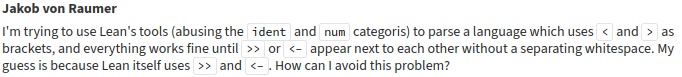
\includegraphics[width=0.8\textwidth]{jakob}
%
%   \bigskip
%   \pause
%   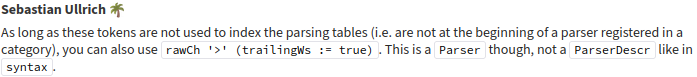
\includegraphics[width=0.8\textwidth]{jakob2}
%\end{frame}

\begin{frame}[fragile]{Embedding Languages in Action}%
  \vspace{-7mm}
  \begin{minipage}[t]{0.5\linewidth}%
\begin{leancode}
declare_syntax_cat jsxElement
declare_syntax_cat jsxChild

syntax jsxAttrName := rawIdent <|> str
syntax jsxAttrVal := str <|> group("{" term "}")
syntax jsxSimpleAttr := jsxAttrName "=" jsxAttrVal
syntax jsxAttrSpread := "[" term "]"
syntax jsxAttr := jsxSimpleAttr <|> jsxAttrSpread

syntax "<" rawIdent jsxAttr* "/>" : jsxElement
syntax "<" rawIdent jsxAttr* ">" jsxChild* "</" rawIdent ">" : jsxElement

syntax jsxText      : jsxChild
syntax "{" term "}" : jsxChild
syntax jsxElement   : jsxChild

scoped syntax:max jsxElement : term
\end{leancode}
  \end{minipage}
  \begin{minipage}[t]{0.45\linewidth}%
\begin{leancode}
macro_rules
  | `(<$n $attrs* />) => do
    let kind := quote (toString n.getId)
    let attrs ← translateAttrs attrs
    `(Html.element $kind true $attrs #[])
  | `(<$n $attrs* >$children*</$m>) => ...
\end{leancode}
\begin{leancode}
def classInstancesToHtml (className : Name) : HtmlM Html := do
  pure
    <details «class»="instances">
        <summary>Instances</summary>
        <ul id={s!"instances-list-{className}"} class="instances-list"></ul>
    </details>
\end{leancode}
  \end{minipage}\\
  \footnotesize{\url{https://github.com/leanprover/doc-gen4}}
\end{frame}

\begin{frame}{Conclusion}
  Arbitrarily extend the Lean grammar using combinator, Pratt, Packrat parsers

  \bigskip

  Extend Lean with other languages... with some current caveats
\end{frame}
\end{document}

%%% Local Variables:
%%% mode: latex
%%% TeX-master: t
%%% TeX-engine: xetex
%%% TeX-command-extra-options: "-shell-escape"
%%% End:
